% =====================================================================
% Lecture 15 - OpenClaw: Building & Understanding Personal AI Agents
% Beamer slides | compile with: pdflatex (run via latexmk -pdf)
% All graphics are TikZ-native (no external image files required).
% =====================================================================
\documentclass[aspectratio=169,11pt]{beamer}

\usepackage[utf8]{inputenc}
\usepackage[T1]{fontenc}
\usepackage{lmodern}
\usepackage{booktabs}
\usepackage{tikz}
\usetikzlibrary{positioning,arrows.meta,shapes.geometric,calc,backgrounds}

% Full-bleed banners/rules intentionally exceed the text block; allow it quietly.
\hfuzz=80pt

% ---------------------------------------------------------------------
% Color palette (lobster theme)
% ---------------------------------------------------------------------
\definecolor{clawDark}{RGB}{33,37,43}
\definecolor{clawOrange}{RGB}{230,81,0}
\definecolor{clawRed}{RGB}{198,40,40}
\definecolor{clawTeal}{RGB}{0,121,107}
\definecolor{clawBlue}{RGB}{21,101,192}
\definecolor{clawGray}{RGB}{117,117,117}
\definecolor{clawLight}{RGB}{245,246,248}

% ---------------------------------------------------------------------
% Clean modern theme (built on default; no external fonts needed)
% ---------------------------------------------------------------------
\usetheme{default}
\usefonttheme{professionalfonts}
\setbeamertemplate{navigation symbols}{}
\setbeamercolor{normal text}{fg=clawDark}
\setbeamercolor{structure}{fg=clawOrange}
\setbeamercolor{alerted text}{fg=clawRed}
\setbeamercolor{title}{fg=clawDark}
\setbeamercolor{frametitle}{fg=white,bg=clawDark}
\setbeamercolor{itemize item}{fg=clawOrange}
\setbeamercolor{itemize subitem}{fg=clawTeal}
\setbeamercolor{block title}{fg=white,bg=clawOrange}
\setbeamercolor{block body}{fg=clawDark,bg=clawLight}
\setbeamercolor{section in toc}{fg=clawDark}
\setbeamerfont{frametitle}{series=\bfseries}
\setbeamerfont{title}{series=\bfseries,size=\huge}
\setbeamertemplate{itemize item}{\small\raise0.5pt\hbox{\textbullet}}

% Frame title with a thin orange rule underneath
\setbeamertemplate{frametitle}{%
  \nointerlineskip
  \begin{beamercolorbox}[wd=\paperwidth,ht=2.6ex,dp=1.2ex,leftskip=0.3cm]{frametitle}%
    \usebeamerfont{frametitle}\insertframetitle%
  \end{beamercolorbox}%
  {\color{clawOrange}\rule{\paperwidth}{1.2pt}}%
}

% Footline: course | title | frame number
\setbeamertemplate{footline}{%
  \leavevmode%
  \hbox{%
    \begin{beamercolorbox}[wd=.33\paperwidth,ht=2.4ex,dp=1ex,leftskip=.3cm]{author in head/foot}%
      \usebeamerfont{author in head/foot}\color{clawGray}\scriptsize Data Science with Python%
    \end{beamercolorbox}%
    \begin{beamercolorbox}[wd=.49\paperwidth,ht=2.4ex,dp=1ex,center]{title in head/foot}%
      \usebeamerfont{title in head/foot}\color{clawGray}\scriptsize Lecture 15 — OpenClaw%
    \end{beamercolorbox}%
    \begin{beamercolorbox}[wd=.15\paperwidth,ht=2.4ex,dp=1ex,rightskip=.3cm]{date in head/foot}%
      \usebeamerfont{date in head/foot}\hfill\color{clawGray}\scriptsize\insertframenumber\,/\,\inserttotalframenumber%
    \end{beamercolorbox}%
  }%
  \vskip0pt%
}

% Section divider slides
\AtBeginSection[]{%
  \begin{frame}[plain,noframenumbering]
    \centering
    \vfill
    {\color{clawOrange}\rule{0.18\paperwidth}{2pt}}\\[1ex]
    {\usebeamerfont{title}\color{clawDark}\insertsectionhead}\\[1ex]
    {\color{clawOrange}\rule{0.18\paperwidth}{2pt}}
    \vfill
  \end{frame}
}

% ---------------------------------------------------------------------
% Reusable TikZ claw icon
% ---------------------------------------------------------------------
\newcommand{\clawicon}[1]{%
\begin{tikzpicture}[scale=#1,line cap=round,line join=round]
  % arm
  \draw[clawOrange,line width=5pt] (-0.2,-0.5) -- (0.55,0.15);
  % upper pincer (open)
  \draw[clawOrange,line width=5pt] (0.55,0.15) .. controls (1.35,0.95) and (1.85,0.35) .. (1.35,-0.05);
  % lower pincer (open)
  \draw[clawOrange,line width=5pt] (0.55,0.15) .. controls (1.15,-0.45) and (1.7,-0.45) .. (1.4,-0.1);
  % pivot
  \fill[clawDark] (0.55,0.15) circle (2.2pt);
\end{tikzpicture}%
}

\title{OpenClaw}
\subtitle{Building \& Understanding Personal AI Agents}
\author{Prof. Alexander Quispe}
\institute{Pontificia Universidad Cat\'olica del Per\'u}
\date{Lecture 15 \,\textbar\, 2026}

% =====================================================================
\begin{document}

% ---------------- TITLE SLIDE ----------------
\begin{frame}[plain,noframenumbering]
  \centering
  \vfill
  {\clawicon{1.6}}\\[1.5ex]
  {\usebeamerfont{title}\color{clawDark}\textbf{open}\textcolor{clawOrange}{claw}}\\[0.6ex]
  {\large\color{clawGray}Building \& Understanding Personal AI Agents}\\[2.2ex]
  {\color{clawOrange}\rule{0.45\paperwidth}{1pt}}\\[1.4ex]
  {\normalsize\color{clawDark}Prof. Alexander Quispe \quad\textbar\quad Data Science with Python}\\[0.4ex]
  {\small\color{clawGray}Pontificia Universidad Cat\'olica del Per\'u \,\textbar\, Lecture 15 \,\textbar\, 2026}
  \vfill
\end{frame}

% ---------------- DISAMBIGUATION ----------------
\begin{frame}{First: which ``OpenClaw''?}
  \begin{columns}[T]
    \begin{column}{0.48\textwidth}
      \begin{block}{\textcolor{white}{This lecture}}
        \textbf{OpenClaw — the AI agent}\\[0.5ex]
        Open-source autonomous assistant by Peter Steinberger. Runs on
        your machine, talks through messaging apps, driven by an LLM.
      \end{block}
    \end{column}
    \begin{column}{0.48\textwidth}
      \begin{block}{\textcolor{white}{NOT this}}
        \textbf{OpenClaw — the game engine}\\[0.5ex]
        A C++ reimplementation of the 1997 platformer \emph{Captain Claw}.
        Same name, totally unrelated.
      \end{block}
    \end{column}
  \end{columns}
  \vspace{1em}
  \begin{center}
    \alert{If you Google ``OpenClaw'' you will hit both — we mean the agent.}
  \end{center}
\end{frame}

% ---------------- OBJECTIVES ----------------
\begin{frame}{Learning objectives}
  By the end of today you will be able to:
  \begin{enumerate}
    \item Explain what an \textbf{autonomous LLM agent} is, and how it differs from a chatbot.
    \item Describe OpenClaw's \textbf{local-first, model-agnostic, channel-based} architecture.
    \item Install and run a minimal instance and connect one messaging channel.
    \item Build \& publish a \textbf{Skill}, and decide \emph{Skill vs.\ MCP server}.
    \item Critically assess the \textbf{security \& privacy risks} of agentic software.
    \item Relate these skills to \textbf{real data-science workflows}.
  \end{enumerate}
\end{frame}

% ---------------- AGENDA ----------------
\begin{frame}{Agenda — 90 minutes}
  \centering
  \renewcommand{\arraystretch}{1.25}
  \begin{tabular}{c l c}
    \toprule
    \textbf{\#} & \textbf{Segment} & \textbf{Min} \\
    \midrule
    1 & Hook: the viral story \& what OpenClaw is & 10 \\
    2 & Concepts: agents vs.\ chatbots; architecture & 20 \\
    3 & \textcolor{clawOrange}{Live demo}: install $\to$ onboard $\to$ connect a channel & 20 \\
    4 & Skills \& ClawHub; Skills vs.\ MCP; build one & 15 \\
    5 & Security, ethics \& failure cases & 15 \\
    6 & Landscape, your use cases, assignment & 10 \\
    \bottomrule
  \end{tabular}
\end{frame}

% =====================================================================
\section{The Story}
% =====================================================================

\begin{frame}{The fastest-growing repo (almost) ever}
  \begin{columns}[T]
    \begin{column}{0.55\textwidth}
      \begin{itemize}
        \item Built by \textbf{Peter Steinberger}, an Austrian developer.
        \item Released \textbf{Nov 24, 2025} as \emph{Clawdbot}.
        \item Renamed twice in two months (trademark + taste).
        \item $\sim$\textbf{247{,}000 GitHub stars} and $\sim$47{,}700 forks by early March 2026.
        \item Steinberger \textbf{joined OpenAI} (Feb 14, 2026); project continues under a non-profit foundation.
      \end{itemize}
    \end{column}
    \begin{column}{0.45\textwidth}
      \centering
      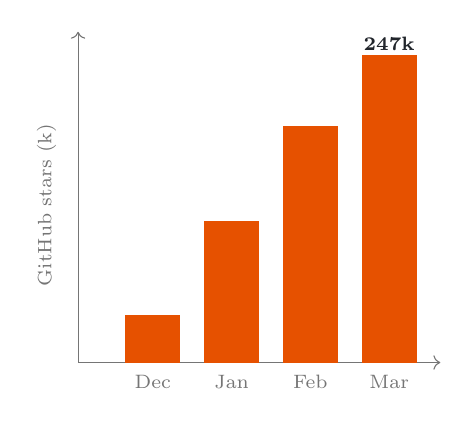
\begin{tikzpicture}[scale=1]
        \def\bw{0.7}
        % axis
        \draw[clawGray,->] (0,0) -- (0,4.2);
        \draw[clawGray,->] (0,0) -- (4.6,0);
        \node[rotate=90,clawGray,font=\scriptsize] at (-0.4,2) {GitHub stars (k)};
        % bars: months Dec, Jan, Feb, Mar
        \foreach \x/\h/\lbl in {0.6/0.6/Dec, 1.6/1.8/Jan, 2.6/3.0/Feb, 3.6/3.9/Mar} {
          \fill[clawOrange] (\x,0) rectangle (\x+\bw,\h);
          \node[clawGray,font=\scriptsize] at (\x+\bw/2,-0.25) {\lbl};
        }
        \node[clawDark,font=\scriptsize\bfseries] at (3.95,4.05) {247k};
      \end{tikzpicture}
      \\[0.4ex]{\scriptsize\color{clawGray}Stars over Dec'25–Mar'26 (illustrative)}
    \end{column}
  \end{columns}
\end{frame}

\begin{frame}{A naming saga (a useful timeline)}
  \centering
  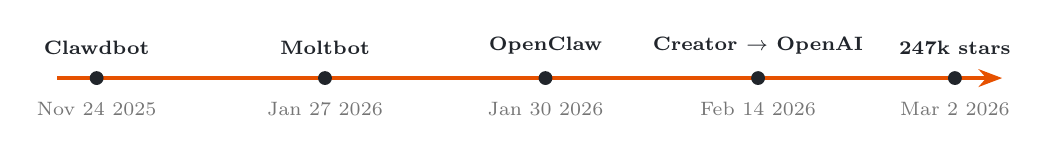
\begin{tikzpicture}[font=\footnotesize]
    \draw[clawOrange,line width=1.2pt,-{Stealth[length=3mm]}] (0,0) -- (12,0);
    \foreach \x/\date/\name in {
      0.5/Nov 24 2025/Clawdbot,
      3.4/Jan 27 2026/Moltbot,
      6.2/Jan 30 2026/OpenClaw,
      8.9/Feb 14 2026/{Creator $\to$ OpenAI},
      11.4/Mar 2 2026/{247k stars}} {
        \fill[clawDark] (\x,0) circle (2.5pt);
        \node[above,clawDark,font=\scriptsize\bfseries,align=center] at (\x,0.18) {\name};
        \node[below,clawGray,font=\scriptsize] at (\x,-0.18) {\date};
    }
  \end{tikzpicture}
  \vspace{1.5em}
  \begin{itemize}
    \item \emph{Clawdbot} $\to$ \emph{Moltbot} after Anthropic trademark complaints.
    \item \emph{Moltbot} $\to$ \emph{OpenClaw} because the name ``never rolled off the tongue.''
  \end{itemize}
\end{frame}

\begin{frame}{What is OpenClaw, in one line?}
  \begin{block}{Definition}
    A \textbf{free, open-source, self-hosted AI agent} that runs on \emph{your}
    machine and talks to you through the messaging apps you already use.
  \end{block}
  \vspace{0.5em}
  \textbf{Channels it speaks on (20+):}
  \begin{center}
    WhatsApp \,\textbullet\, Telegram \,\textbullet\, Slack \,\textbullet\, Discord \,\textbullet\, Signal \,\textbullet\,
    iMessage \\ Microsoft Teams \,\textbullet\, Matrix \,\textbullet\, Google Chat \,\textbullet\, IRC \,\textbullet\, WeChat \,\textbullet\, \ldots
  \end{center}
  \vspace{0.5em}
  \begin{center}
    \textcolor{clawOrange}{\textbf{Key shift:}} from an LLM that \emph{answers} $\;\to\;$ an LLM that \emph{acts}.
  \end{center}
\end{frame}

% =====================================================================
\section{Concepts \& Architecture}
% =====================================================================

\begin{frame}{Chatbot vs.\ agent}
  \centering
  \renewcommand{\arraystretch}{1.3}
  \begin{tabular}{l l}
    \toprule
    \textbf{Chatbot} & \textbf{Agent} \\
    \midrule
    Returns text & Plans, acts, observes, remembers \\
    Stateless turn & Maintains memory \& goals \\
    No side effects & Calls tools / APIs, executes actions \\
    ``What is X?'' & ``Do X, then tell me on Discord'' \\
    \bottomrule
  \end{tabular}
  \vspace{1.2em}
  \begin{center}
    The agent runs a \textbf{loop}, not a single reply.
  \end{center}
\end{frame}

\begin{frame}{The agent loop}
  \centering
  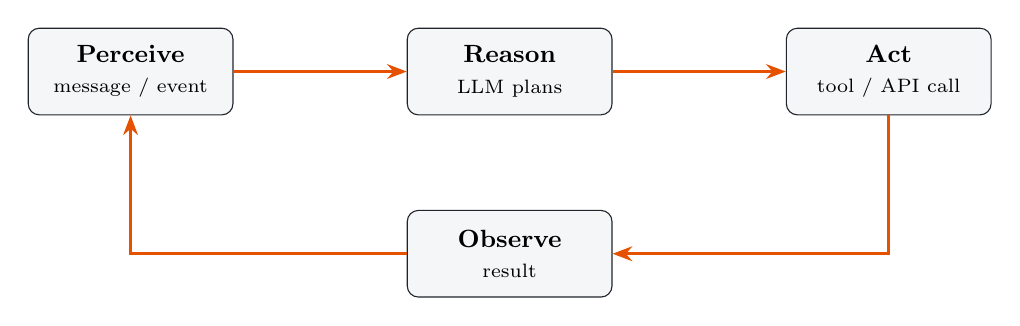
\begin{tikzpicture}[
      node distance=12mm and 22mm,
      box/.style={draw=clawDark,fill=clawLight,rounded corners,minimum width=26mm,minimum height=11mm,align=center,font=\small\bfseries},
      arr/.style={-{Stealth[length=2.5mm]},clawOrange,line width=1pt}]
    \node[box] (p) {Perceive\\{\scriptsize\mdseries message / event}};
    \node[box,right=of p] (r) {Reason\\{\scriptsize\mdseries LLM plans}};
    \node[box,right=of r] (a) {Act\\{\scriptsize\mdseries tool / API call}};
    \node[box,below=of r] (o) {Observe\\{\scriptsize\mdseries result}};
    \draw[arr] (p) -- (r);
    \draw[arr] (r) -- (a);
    \draw[arr] (a) |- (o);
    \draw[arr] (o) -| (p);
    \node[clawGray,font=\scriptsize] at (r |- o) {} ;
  \end{tikzpicture}
  \vspace{0.8em}
  \begin{center}
    The LLM is the \emph{brain}; tools are the \emph{hands}; memory is \emph{continuity}.
  \end{center}
\end{frame}

\begin{frame}{Four design principles}
  \begin{columns}[T]
    \begin{column}{0.5\textwidth}
      \begin{block}{Local-first}
        Runs on your hardware; your data stays with you instead of going to a vendor first.
      \end{block}
      \begin{block}{Model-agnostic}
        Plug in Claude, GPT, Gemini, DeepSeek — not locked to one provider.
      \end{block}
    \end{column}
    \begin{column}{0.5\textwidth}
      \begin{block}{Channel-based UI}
        No custom app — the interface is a chat thread in apps you already use.
      \end{block}
      \begin{block}{Extensible}
        \textbf{Skills} (plain-language) + \textbf{MCP} servers (standard tool protocol).
      \end{block}
    \end{column}
  \end{columns}
\end{frame}

\begin{frame}{Architecture at a glance}
  \centering
  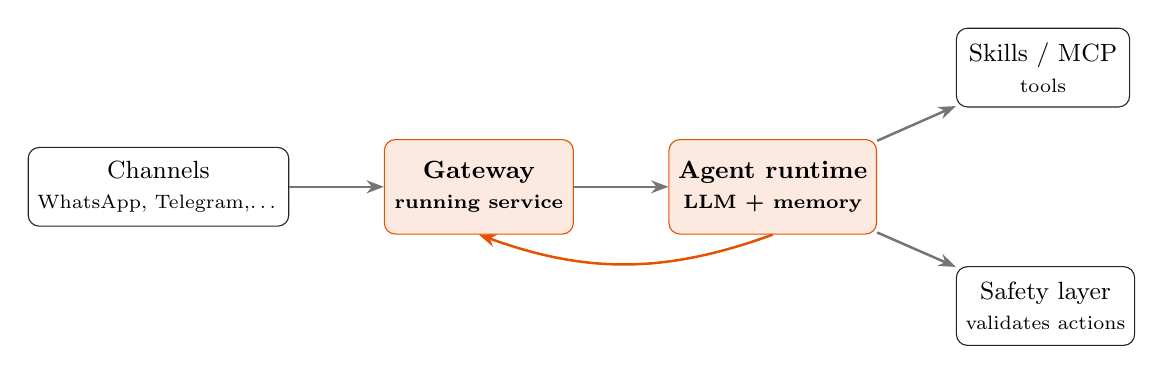
\begin{tikzpicture}[
      node distance=7mm and 12mm,
      comp/.style={draw=clawDark,fill=white,rounded corners,minimum height=10mm,align=center,font=\small},
      core/.style={draw=clawOrange,fill=clawOrange!12,rounded corners,minimum height=12mm,align=center,font=\small\bfseries},
      arr/.style={-{Stealth[length=2.2mm]},clawGray,line width=0.9pt}]
    \node[comp,minimum width=24mm] (chan) {Channels\\{\scriptsize WhatsApp, Telegram,\ldots}};
    \node[core,right=of chan,minimum width=24mm] (gw) {Gateway\\{\scriptsize running service}};
    \node[core,right=of gw,minimum width=26mm] (rt) {Agent runtime\\{\scriptsize LLM + memory}};
    \node[comp,above right=4mm and 10mm of rt,minimum width=22mm] (sk) {Skills / MCP\\{\scriptsize tools}};
    \node[comp,below right=4mm and 10mm of rt,minimum width=22mm] (sf) {Safety layer\\{\scriptsize validates actions}};
    \draw[arr] (chan) -- (gw);
    \draw[arr] (gw) -- (rt);
    \draw[arr] (rt) -- (sk);
    \draw[arr] (rt) -- (sf);
    \draw[arr,clawOrange] (rt.south) to[bend left=20] (gw.south);
  \end{tikzpicture}
  \vspace{0.6em}
  \begin{center}
    \scriptsize Message $\to$ Gateway $\to$ runtime reasons $\to$ calls a tool $\to$ safety check $\to$ reply.
  \end{center}
\end{frame}

\begin{frame}{Tech stack \& requirements}
  \begin{columns}[T]
    \begin{column}{0.5\textwidth}
      \textbf{Built with}
      \begin{itemize}
        \item TypeScript (core) + Swift (Apple clients)
        \item Local config files (the ``local-first'' part you can inspect)
        \item Runs on Windows, macOS, Linux
      \end{itemize}
    \end{column}
    \begin{column}{0.5\textwidth}
      \textbf{You need}
      \begin{itemize}
        \item \textbf{Node.js $\geq$ 22}
        \item An API key: Anthropic / OpenAI / Google
        \item A messaging account to connect (use a \alert{test} one!)
      \end{itemize}
    \end{column}
  \end{columns}
  \vspace{1em}
  \begin{center}
    \scriptsize\color{clawGray}Connects back to Lecture 11 (ModernBERT) \& Lecture 13 (fine-tuning):
    the ``brain'' is the same kind of model you have already used.
  \end{center}
\end{frame}

% =====================================================================
\section{Live Demo}
% =====================================================================

\begin{frame}[fragile]{Live demo — zero to assistant}
  \textbf{Install (one of):}
\begin{verbatim}
  npx clawdbot@latest
  # or
  curl -fsSL https://openclaw.ai/install.sh | bash
\end{verbatim}
  \textbf{Then:}
  \begin{enumerate}
    \item Run onboarding $\to$ paste an API key $\to$ pick a model.
    \item Connect \emph{one} channel (Telegram bot token or Discord = easiest live).
    \item Send the first message; watch it reason and reply.
    \item Open the config files on disk — see ``local-first'' for real.
  \end{enumerate}
\end{frame}

\begin{frame}{Demo safety rules (do this every time)}
  \begin{itemize}
    \item Run it in a \textbf{VM / container}, not your daily machine.
    \item Use a \textbf{dedicated API key with a spend cap}.
    \item Use a \textbf{throwaway} Telegram/Discord account.
    \item \alert{Never} grant full-disk or terminal access where real secrets live.
  \end{itemize}
  \vspace{1em}
  \begin{block}{Why so cautious?}
    An agent that can run commands and read files turns a small bug into a
    big breach. We will see exactly how in the security segment.
  \end{block}
\end{frame}

% =====================================================================
\section{Skills \& ClawHub}
% =====================================================================

\begin{frame}{Skills = apps for your agent}
  \begin{itemize}
    \item A \textbf{Skill} = a \texttt{SKILL.md} (plain-language instructions) + supporting files.
    \item \textbf{ClawHub} = the public registry — \textbf{13{,}700+} community skills (late Feb 2026).
    \item Mental model: \emph{OpenClaw is the OS; skills are the apps you install.}
  \end{itemize}
  \vspace{0.8em}
  \begin{center}
  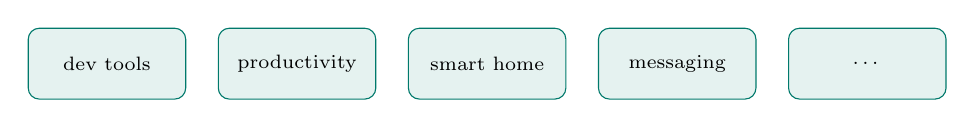
\begin{tikzpicture}[font=\scriptsize,
      app/.style={draw=clawTeal,fill=clawTeal!10,rounded corners,minimum width=20mm,minimum height=9mm,align=center}]
    \node[app] (a) {dev tools};
    \node[app,right=4mm of a] (b) {productivity};
    \node[app,right=4mm of b] (c) {smart home};
    \node[app,right=4mm of c] (d) {messaging};
    \node[app,right=4mm of d] (e) {\ldots};
  \end{tikzpicture}
  \end{center}
\end{frame}

\begin{frame}{Skill vs.\ MCP server — when to use which}
  \centering
  \renewcommand{\arraystretch}{1.3}
  \begin{tabular}{l l}
    \toprule
    \textbf{Skill} & \textbf{MCP server} \\
    \midrule
    Plain-language instructions & Separate process exposing tools \\
    Read by the agent at runtime & Standard protocol (MCP) \\
    OpenClaw-specific & Portable: Claude Desktop, Cursor, VS Code\ldots \\
    Fastest for one automation & Best for state / many tool endpoints \\
    \bottomrule
  \end{tabular}
  \vspace{1.0em}
  \begin{center}
    \textcolor{clawOrange}{\textbf{Best of both:}} build an \emph{MCP server} for the capability,
    wrap it in a \emph{Skill} for the workflow.
  \end{center}
\end{frame}

\begin{frame}[fragile]{Building \& publishing a Skill}
  A minimal \texttt{SKILL.md}:
\begin{verbatim}
  ---
  name: daily-arxiv-digest
  description: Summarize new arXiv papers on a topic each morning
  ---
  When asked for my digest:
  1. Fetch today's arXiv listing for the given category.
  2. Summarize the 5 most relevant titles in 2 lines each.
  3. Send the summary to me on Telegram.
\end{verbatim}
  \textbf{Publish:} fork \texttt{github.com/openclaw/clawhub} $\to$ add your folder $\to$
  open a PR. \scriptsize(GitHub account must be $\geq$ 1 week old.)
\end{frame}

% =====================================================================
\section{Security \& Ethics}
% =====================================================================

\begin{frame}{Why the stakes are high}
  \begin{block}{The agent can touch everything}
    Local files \,\textbullet\, browser state \,\textbullet\, SaaS sessions \,\textbullet\, OAuth tokens \,\textbullet\, command execution.
  \end{block}
  \vspace{0.6em}
  A bug here is not a wrong answer — it is \alert{data theft or remote code execution}.
  \vspace{0.8em}
  \begin{itemize}
    \item Feb 2026: \textbf{40{,}214} internet-exposed instances observed (SecurityScorecard); $\sim$35\% flagged vulnerable.
    \item Thousands susceptible to remote code execution in early scans.
  \end{itemize}
\end{frame}

\begin{frame}{Notable 2026 CVEs (case studies)}
  \centering
  \renewcommand{\arraystretch}{1.25}
  \begin{tabular}{l l l}
    \toprule
    \textbf{CVE} & \textbf{Type} & \textbf{Note} \\
    \midrule
    2026-32922 & Privilege escalation & CVSS \textbf{9.9}; \texttt{device.token.rotate} \\
    2026-25253 & Token leak & auto-connect to attacker \texttt{gatewayUrl} \\
    2026-24763 & Command injection & \\
    2026-26322 & SSRF & \\
    2026-26329 & Path traversal & local file reads \\
    2026-30741 & Prompt-injection RCE & via malicious content \\
    \bottomrule
  \end{tabular}
  \vspace{0.8em}
  \begin{center}\scriptsize ``Claw Chain'' (Cyera) chained four flaws $\to$ data theft + persistence.\end{center}
\end{frame}

\begin{frame}{Supply chain: the ``ClawHavoc'' incident}
  \begin{itemize}
    \item Jan 2026: researchers (Koi) found \textbf{341 malicious skills} on ClawHub.
    \item Typosquatted names + fake ``prerequisite'' steps delivered the AMOS macOS stealer, reverse shells, credential exfiltration.
    \item Grew to \textbf{800+} flagged skills by mid-Feb 2026.
  \end{itemize}
  \vspace{1em}
  \begin{block}{The lesson}
    \textbf{Installing a skill = running someone else's code.} Anyone with a
    week-old GitHub account could publish, with little review.
  \end{block}
\end{frame}

\begin{frame}{Hardening checklist (handout)}
  \begin{columns}[T]
    \begin{column}{0.5\textwidth}
      \begin{itemize}
        \item Isolate: VM / container
        \item Least-privilege tokens + spend caps
        \item No broad network binding
        \item Strong authentication
      \end{itemize}
    \end{column}
    \begin{column}{0.5\textwidth}
      \begin{itemize}
        \item Vet every skill's source code
        \item Keep the agent updated
        \item Never run with production secrets present
        \item Log \& review actions
      \end{itemize}
    \end{column}
  \end{columns}
  \vspace{1em}
  \begin{center}
    \textcolor{clawOrange}{\textbf{Convenience and blast radius scale together.}}
  \end{center}
\end{frame}

% =====================================================================
\section{Landscape \& Wrap}
% =====================================================================

\begin{frame}{OpenClaw vs.\ Gemini Spark}
  \centering
  \renewcommand{\arraystretch}{1.25}
  \begin{tabular}{l l l}
    \toprule
     & \textbf{OpenClaw} & \textbf{Gemini Spark} \\
    \midrule
    Hosting & Self-hosted (your box) & Google Cloud, always on \\
    Ease & Needs setup/upkeep & Beginner-friendly \\
    Models & Any (Claude/GPT/Gemini\ldots) & Gemini only \\
    Integrations & MCP $\to$ almost anything & Best inside Google Workspace \\
    Sweet spot & Cross-boundary workflows & Tasks inside Google \\
    \bottomrule
  \end{tabular}
  \vspace{0.7em}
  \begin{center}\scriptsize Others: Anthropic Claude Cowork, OpenAI ChatGPT Agent, managed hosts (MyClaw).\end{center}
\end{frame}

\begin{frame}{How \emph{you} use these skills}
  \begin{itemize}
    \item \textbf{Automate pipelines:} scrape $\to$ clean $\to$ store $\to$ notify.
    \item \textbf{Monitoring agents:} watch a dataset/endpoint, alert on drift or anomalies.
    \item \textbf{Research assistant:} summarize papers \& threads, draft reports.
    \item \textbf{Portfolio project:} a custom Skill + MCP server is a strong, demonstrable artifact.
    \item \textbf{Career:} ``agent engineering'' is emerging — understanding the \emph{security tradeoffs} sets you apart.
  \end{itemize}
\end{frame}

\begin{frame}{Discussion \& assignment}
  \textbf{Discuss:}
  \begin{enumerate}
    \item Why might a university or bank \emph{ban} self-hosted agents? Justified?
    \item When is local-first safer than cloud — and when is it the opposite?
    \item A useful ClawHub skill has 12 stars, no reviews. Install it? How decide?
  \end{enumerate}
  \vspace{0.6em}
  \textbf{Assignment (pick one):}
  \begin{itemize}
    \item[A] \textbf{Build} a minimal Skill (\texttt{SKILL.md} + demo video). \emph{Sandbox required.}
    \item[B] \textbf{Analyze} one CVE $\to$ 1-page threat model (vector, blast radius, fix).
    \item[C] \textbf{Compare} OpenClaw vs.\ Spark vs.\ a plain script for one DS task.
  \end{itemize}
\end{frame}

\begin{frame}{Key resources}
  \footnotesize
  \textbf{Official:} \texttt{docs.openclaw.ai/start/getting-started} \,\textbullet\, \texttt{github.com/openclaw/openclaw} \,\textbullet\, \texttt{github.com/openclaw/clawhub} \,\textbullet\, Wikipedia: ``OpenClaw''\\[0.6ex]
  \textbf{Tutorials:} DataCamp ``Building Custom OpenClaw Skills'' \,\textbullet\, DEV ``Zero to AI Assistant in 10 Minutes'' \,\textbullet\, VoltAgent \texttt{awesome-openclaw-skills}\\[0.6ex]
  \textbf{News/context:} Lex Fridman \#491 (Steinberger) \,\textbullet\, The New Stack ``OpenClaw vs Gemini Spark''\\[0.6ex]
  \textbf{Security:} The Hacker News (four flaws) \,\textbullet\, ARMO (CVE-2026-32922) \,\textbullet\, Microsoft Security Blog (running it safely) \,\textbullet\, Sangfor \,\textbullet\, DigitalOcean\\[1ex]
  \scriptsize\color{clawGray}Many community blogs in this space are AI-generated — verify any exact command/number against the official docs or vendor security pages.
\end{frame}

\begin{frame}[plain,noframenumbering]
  \centering
  \vfill
  {\clawicon{1.3}}\\[1.2ex]
  {\usebeamerfont{title}\color{clawDark}Thank you}\\[0.6ex]
  {\large\color{clawGray}Questions?}\\[1.5ex]
  {\small\color{clawDark}Lecture 15 — OpenClaw \,\textbar\, Data Science with Python}
  \vfill
\end{frame}

\end{document}
